\documentclass{beamer}
\usepackage{graphicx, subfigure}
\usepackage{algorithm, algorithmic}

\usetheme[compress]{Dresden}
\setbeamertemplate{navigation symbols}{} 

\title{Locate My Plate \\ A License Plate Localisation System}
\subtitle{presented by: Tjerk Kostelijk, Folkert Huizinga}
\date{July 1, 2009}

\begin{document}

\frame{\titlepage}

\setcounter{tocdepth}{1}

\frame
{
  \frametitle{Outline}
  \small
  \tableofcontents
  \normalsize
}

\setcounter{tocdepth}{2}

\AtBeginSection[]
{
 \begin{frame}
  \frametitle{Outline}
  \small
  \tableofcontents[currentsection,hideothersubsections]
  \normalsize
 \end{frame}
}

\section{Introduction}
\frame
{
  \frametitle{Introduction}
	
  \begin{itemize}
  \item <+-| alert@+> Implementation License Plate Localisation
  \item <+-| alert@+> Feature Analysis
  \item <+-| alert@+> Cascading Classifier
  \item <+-| alert@+> Strong Classifier
  \item <+-| alert@+> Weak Classifier
  \end{itemize}
}

\section{Features}
\frame
{
  \frametitle{Features}
	
  \begin{itemize}
  \item <+-| alert@+> Image Filter
  \item <+-| alert@+> Image Type
  \item <+-| alert@+> Horizontal or Vertical
  \item <+-| alert@+> Generation using powerset
  \end{itemize}
}

\frame
{
	\begin{figure}[!ht]
		\centering
		\subfigure{
		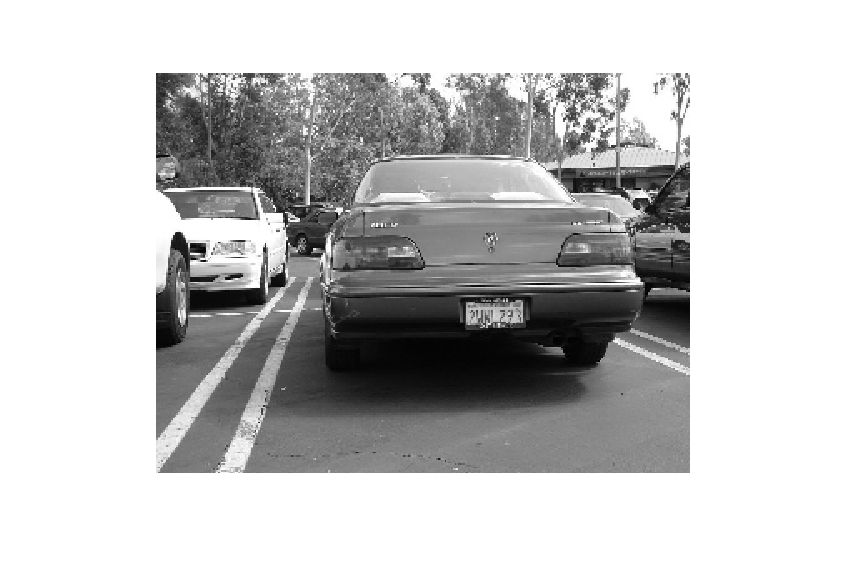
\includegraphics[height=3.5cm]{../report/img/original}
		\label{fig:a}
		}
		\subfigure{
		\includegraphics[height=3.5cm]{../report/img/feature}
		\label{fig:b}
		}
		\subfigure{
		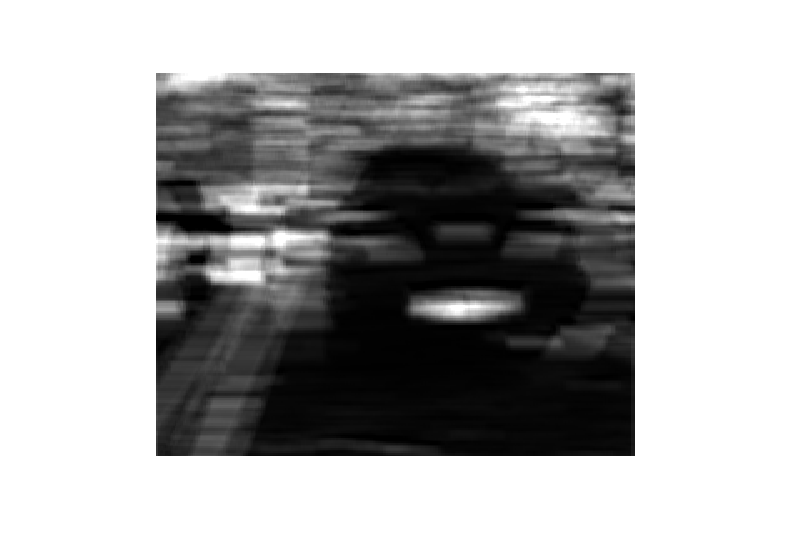
\includegraphics[height=3.5cm]{../report/img/featureapplied}
		\label{fig:c}
		}
		\caption{A horizontal, second order $x$-derivative feature with binary code
		$01110$, consisting of three blocks applied to an image.}
		\label{fig:feature}
	\end{figure}
}

\section{Stage I: Weak}
\frame
{
  \frametitle{Stage I: Weak}
	
  \begin{itemize}
  \item <+-| alert@+> xxx
  \end{itemize}
}

\section{Stage II: Strong}
\frame
{
  \frametitle{Stage II: Strong}
	
  \begin{itemize}
  \item <+-| alert@+> Linear combination of weak classifiers
  \item <+-| alert@+> Training
  \begin{itemize}
  	\item Boosting algorithm
  	\item Alphas
  	\item Weighted samples
  \end{itemize}
  \item <+-| alert@+> Classification
	\begin{displaymath}
	C(x) = 
		\left\{ \begin{array}{ll}
			1 & \sum^N_{i=1} \alpha_i \big(t_i \circ_i f_i(x)\big) \ge \tau \sum^N_{i=1}\alpha_i \\
			0 & \textrm{otherwise}
		\end{array} \right.
	\end{displaymath}
  \end{itemize}
}

\frame
{
	\begin{figure}[!ht]
	\centering
	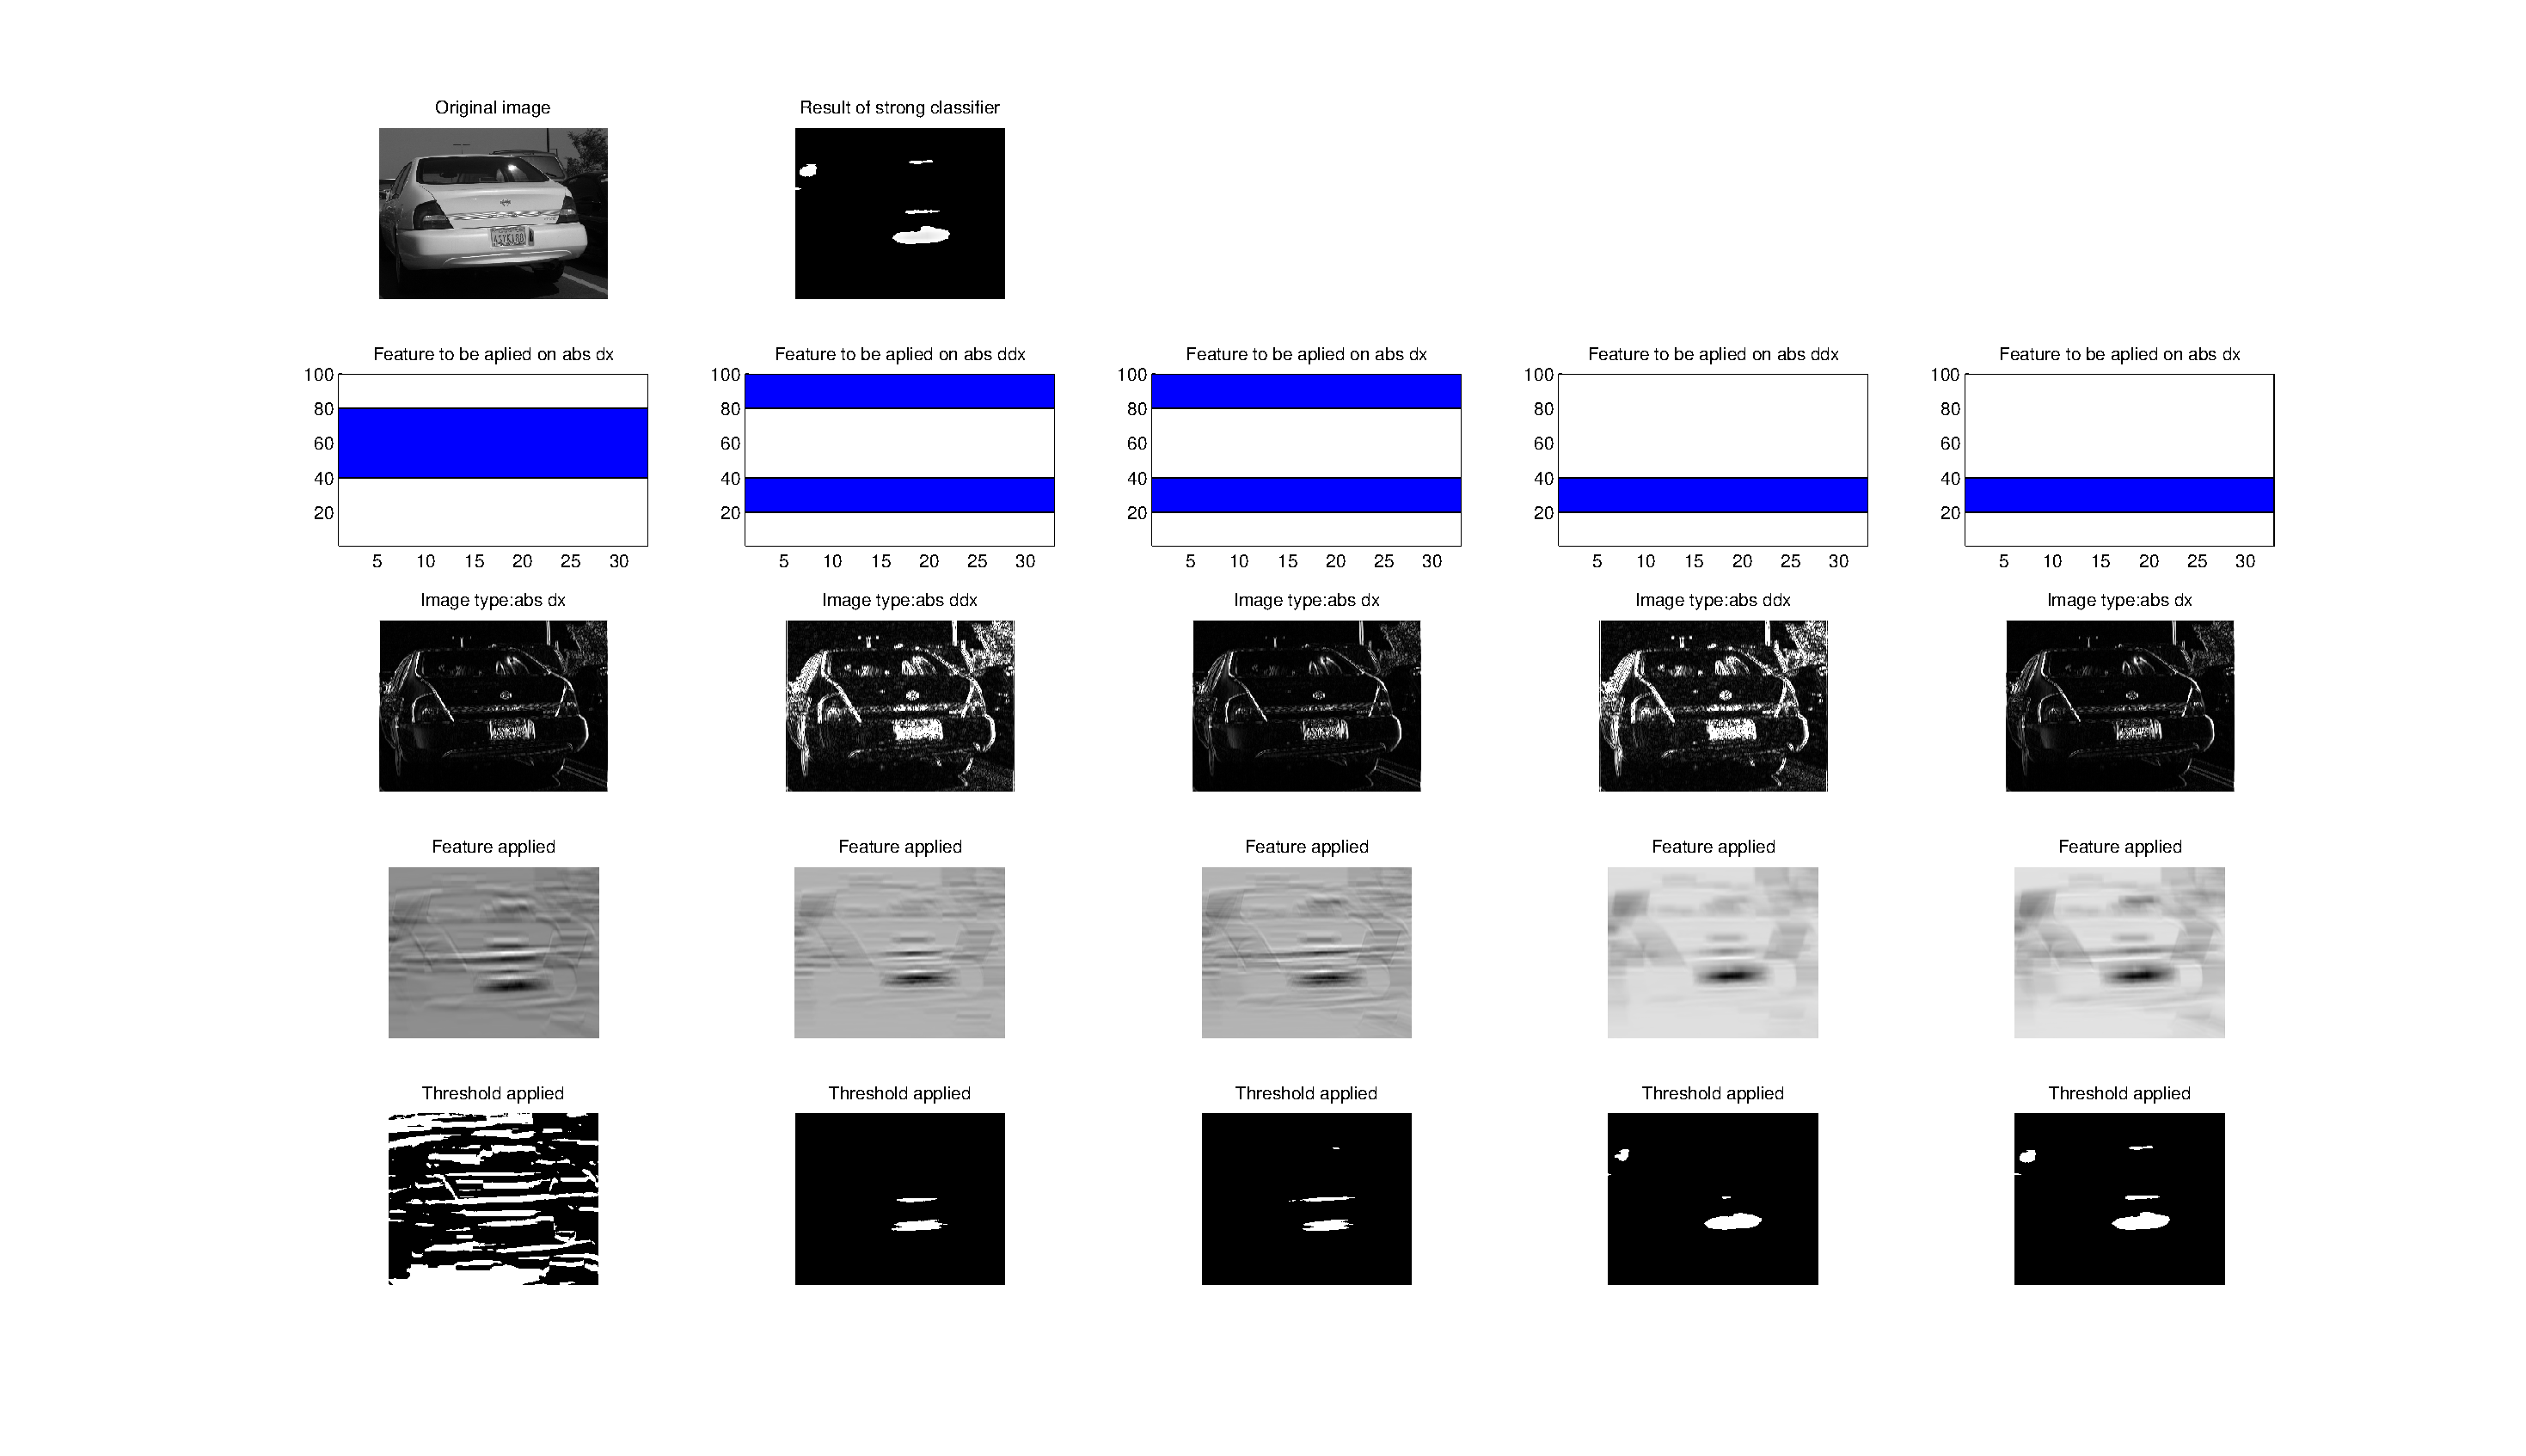
\includegraphics[width=10cm]{../report/img/strongClassifier_layer2_img14}
	\label{fig:strongclassify}
	\end{figure}
}

\section{Stage III: Cascading}
\frame
{
  \frametitle{Stage III: Cascading}
	
  \begin{itemize}
  \item <+-| alert@+> A sequence of strong classifiers
  \item <+-| alert@+> Training
  \begin{itemize}
  	\item False positive rate per layer
  	\item Detection rate per layer
  	\item Desired false positive rate
  	\item Update Negatives using validation set
  \end{itemize}
  \item <+-| alert@+> Classification next slide
  \end{itemize}
}

\frame
{
  \frametitle{Stage III: Cascading}
  \begin{algorithm}[H]
  	\caption{cascadingClassify($C$, $x$, $w$, $h$): Returns the binary image $B$ of $x$}
  	\begin{algorithmic}[1]
  	\REQUIRE $C$ the cascading classifier, $x$ the image, $w,h$ the dimensions of the features
  	\medskip
  	\STATE Initialize $B$ as an image with dimensions $D(x) - [w,h]$ consisting of ones.
  	\FORALL {$c_s \in C$}
  		\STATE $B' \leftarrow c_s(x)$
  		\STATE $B \leftarrow B \land B'$
  	\ENDFOR
  	\RETURN $B$
  	\end{algorithmic}
  \label{alg:casc}
  \end{algorithm}
}

\frame
{
	\begin{figure}[!ht]
	\centering
	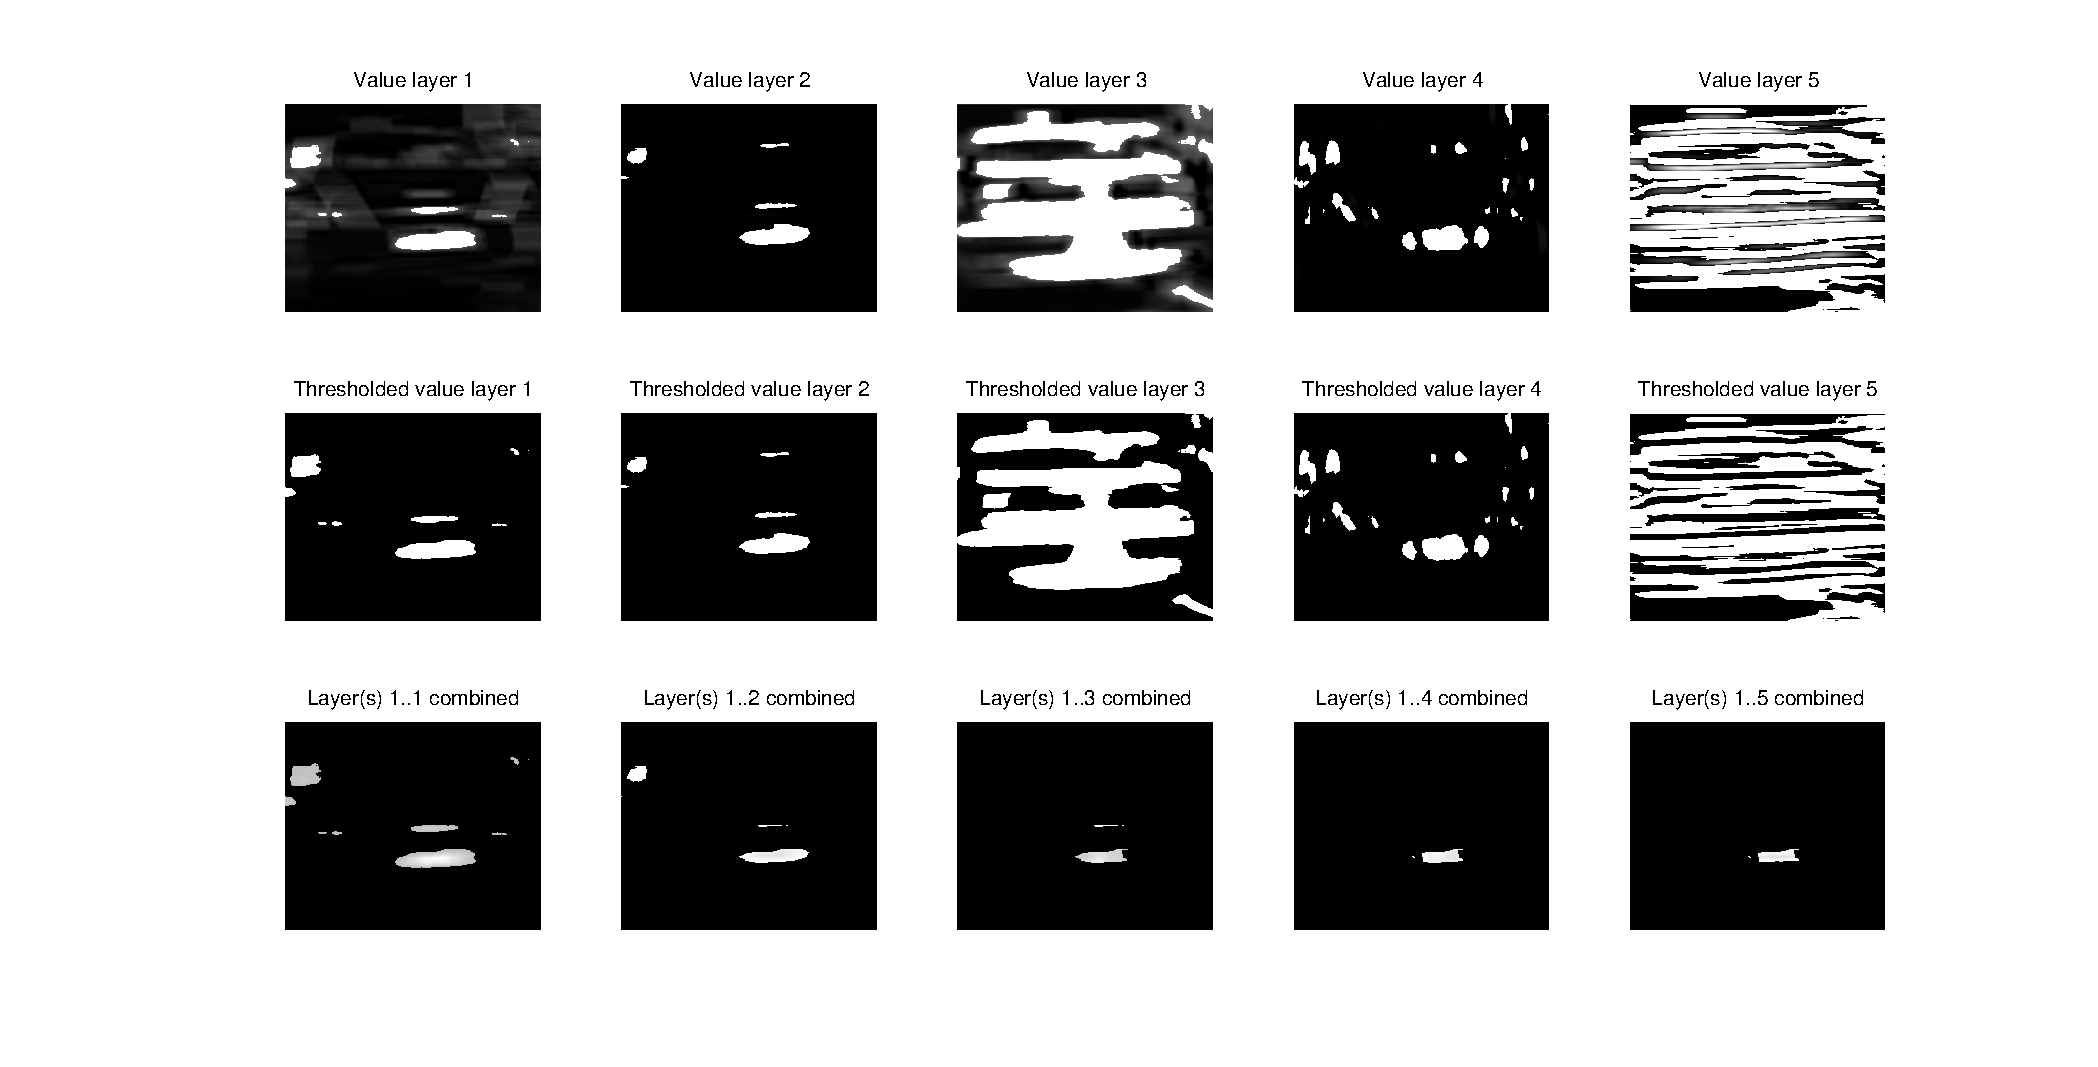
\includegraphics[width=12cm]{../report/img/cascader_img14}
	\label{fig:cascader}
	\end{figure}
}

\section{Results}
\frame
{
  \frametitle{Results}
	
  \begin{itemize}
  \item <+-| alert@+> 4 Image Types
  \item <+-| alert@+> Test Set (47 images)
  \item <+-| alert@+> Detection rate $0.925$
  \item <+-| alert@+> False positive rate $0.065$
  \item <+-| alert@+> Confusion Matrix
  \begin{table}[!ht]
  \centering
  \begin{tabular}{|l|l|}
  \hline
  $37$ & $166186$ \\
  \hline
  $3$  & $2399245$ \\
  \hline
  \end{tabular}
  \caption{Confusion Matrix}
  \label{tab:conf}
  \end{table}
  \end{itemize}
}

\frame
{
  \frametitle{Results}
  \begin{figure}[!ht]
  \centering
  \includegraphics[width=10cm]{../report/img/fprate}
  \end{figure}
}

\frame
{
  \frametitle{Results}
	\begin{figure}[!ht]
	\centering

		\subfigure{
			\includegraphics[width=5cm]{../report/img/cascader_original}
		}
		\subfigure{
			\includegraphics[width=5cm]{../report/img/cascader_result}
		}

	\end{figure}
}

\section{Conclusions}
\frame
{
  \frametitle{Conclusions}
	
  \begin{itemize}
  \item <+-| alert@+> Good results considering 4 image types!
  \item <+-| alert@+> Practical when filtering rest with OCR
  \item <+-| alert@+> Very fast (even in matlab)
  \end{itemize}
}
\end{document}
